\message{ !name(presBellTestInContVar.tex)}%% LyX 2.1.3 created this file.  For more info, see http://www.lyx.org/.
%% Do not edit unless you really know what you are doing.
\documentclass[twocolumn,british]{beamer}
\usepackage{ccfonts}
\renewcommand{\familydefault}{\rmdefault}
\usepackage[T1]{fontenc}
\usepackage[latin9]{inputenc}
\setcounter{secnumdepth}{3}
\setcounter{tocdepth}{3}
\usepackage{amsmath}
\usepackage{amssymb}
\usepackage{graphicx}

\makeatletter

%%%%%%%%%%%%%%%%%%%%%%%%%%%%%% LyX specific LaTeX commands.
%% Because html converters don't know tabularnewline
\providecommand{\tabularnewline}{\\}

%%%%%%%%%%%%%%%%%%%%%%%%%%%%%% Textclass specific LaTeX commands.
 % this default might be overridden by plain title style
 \newcommand\makebeamertitle{\frame{\maketitle}}%
 % (ERT) argument for the TOC
 \AtBeginDocument{%
   \let\origtableofcontents=\tableofcontents
   \def\tableofcontents{\@ifnextchar[{\origtableofcontents}{\gobbletableofcontents}}
   \def\gobbletableofcontents#1{\origtableofcontents}
 }

\makeatother

\usepackage{babel}
\begin{document}

\message{ !name(presBellTestInContVar.tex) !offset(-3) }


\title{Bell Test in phase space (q,p)}
\makebeamertitle
\begin{frame}{Introduction}

\begin{itemize}
\item Programme: DAAD
\item Place: University of Siegen, Siegen\\
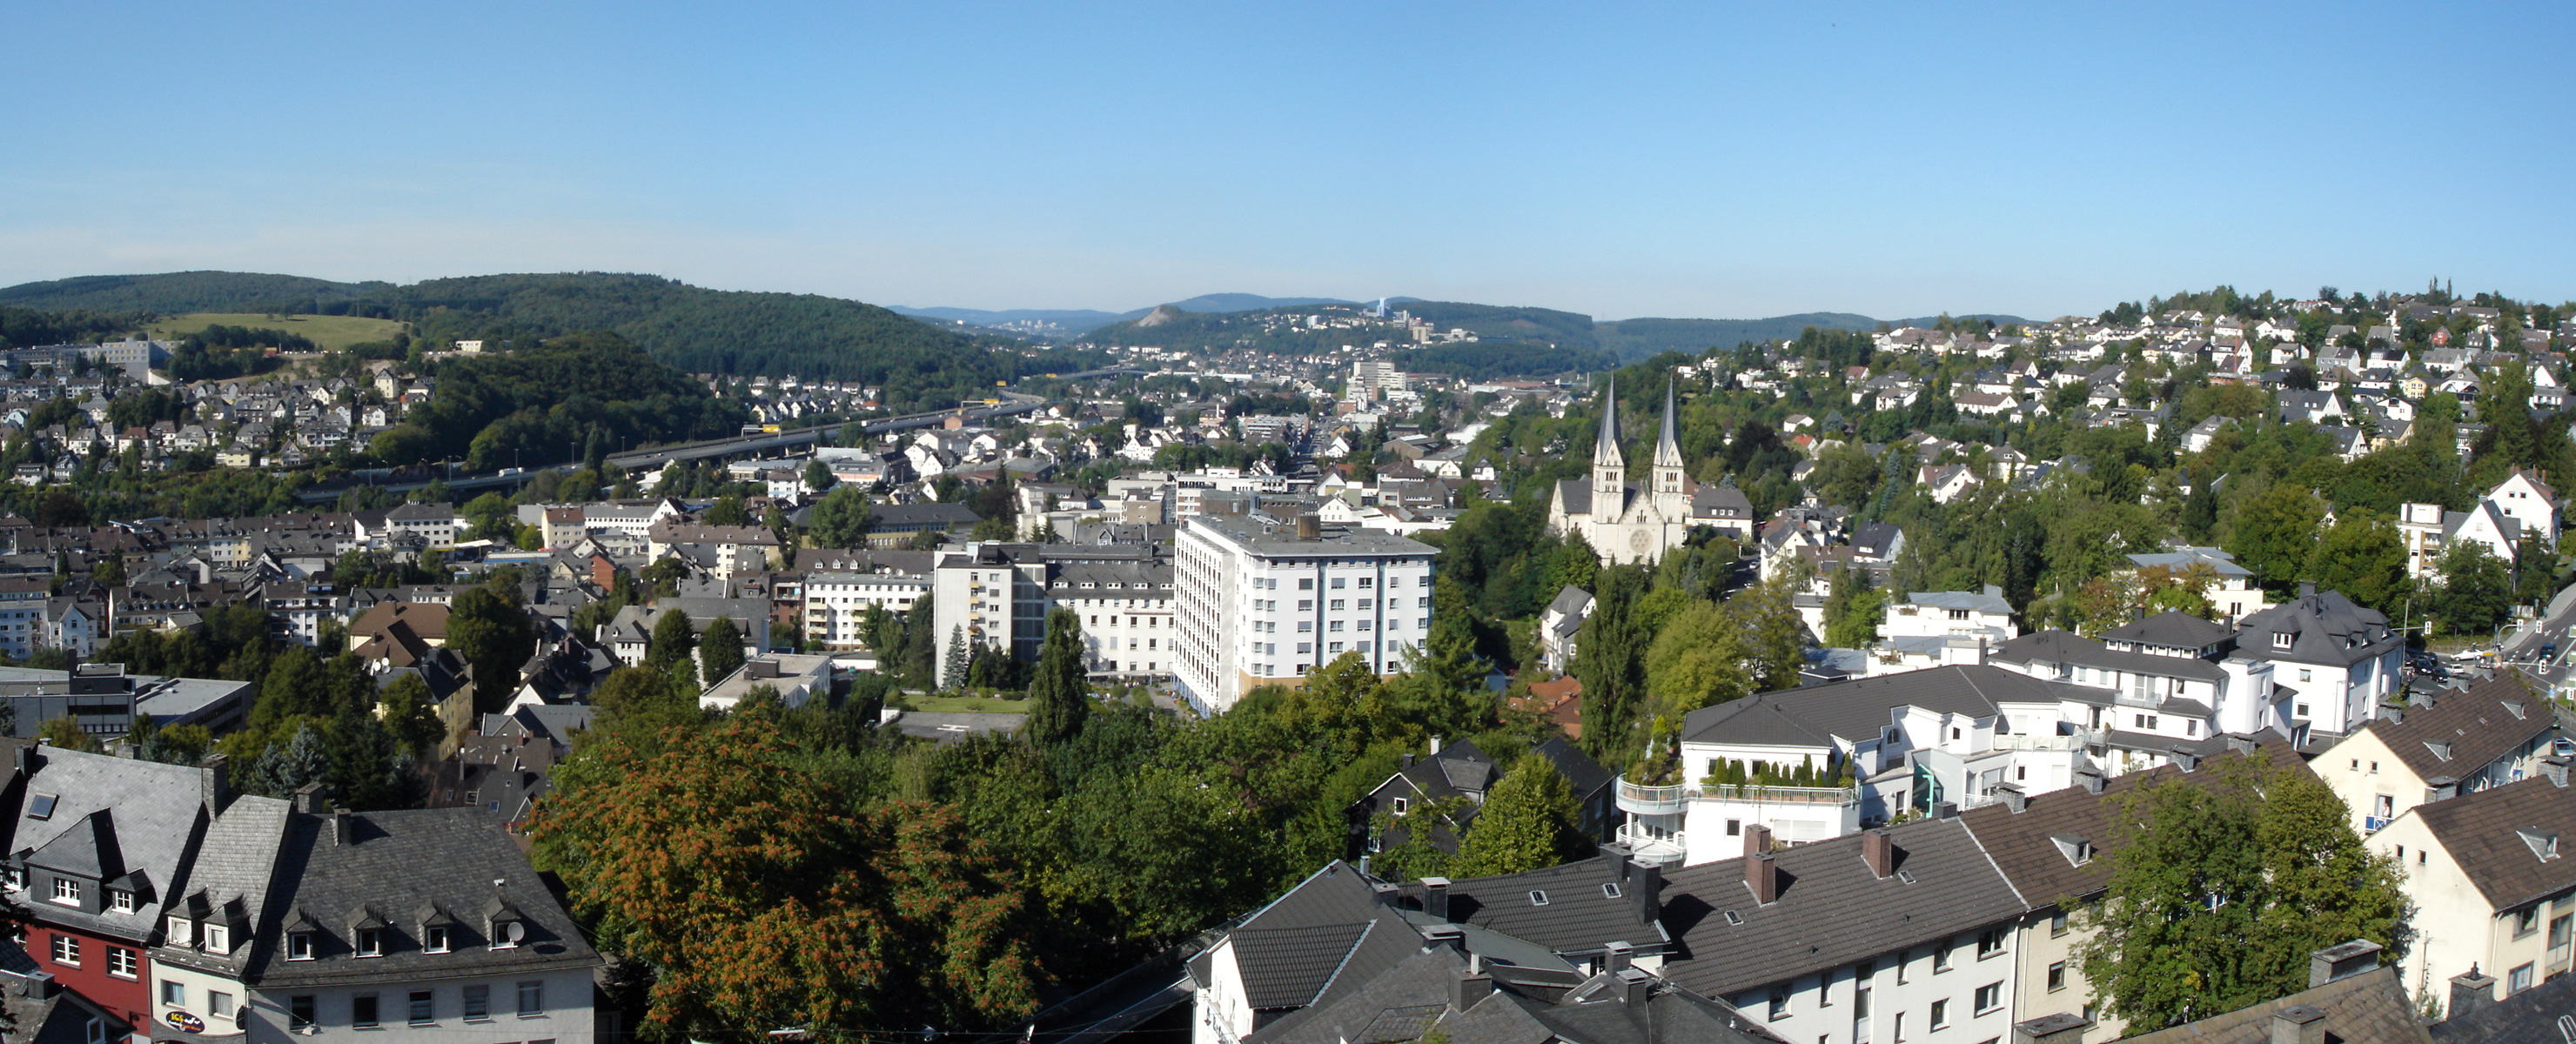
\includegraphics[scale=0.1]{images/siegen}
\item People: Prof. Otfried Guehne and Dr. Ali Assadian\\
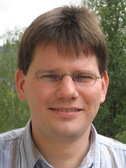
\includegraphics[width=2cm]{images/otfried}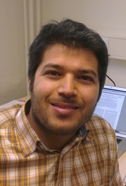
\includegraphics[width=2cm]{images/asadian}
\end{itemize}
\end{frame}

\begin{frame}{}


\Huge{Motivation}
\end{frame}
\begin{section}{Motivation}

\begin{frame}{Mechanics}

\begin{itemize}
\item Newton et. al. : `Classical Mechanics' $\mathbf{q},\mathbf{p}$ \&
forces; t
\item 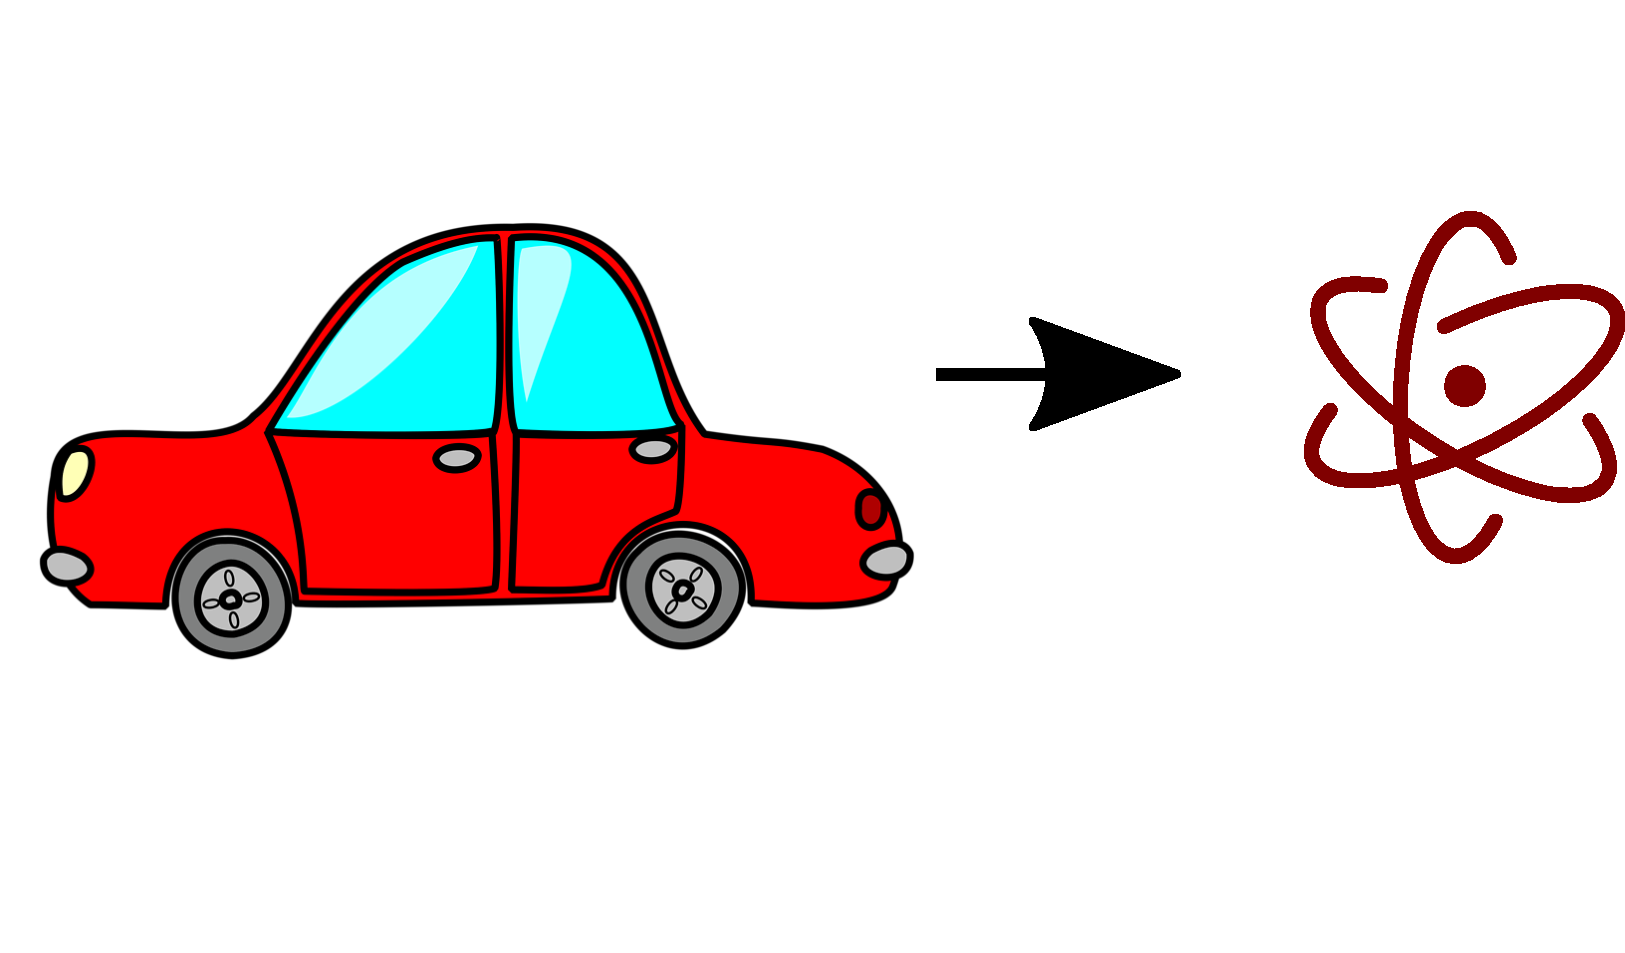
\includegraphics[width=5cm]{images/carToAtom}\cite{car}\cite{atom}
\item Heisenberg, Schr�dinger et. al. : `Quantum Mechanics' $[\hat{\mathbf{q}},\hat{\mathbf{p}}]=i\hbar$
\end{itemize}
\end{frame}

\begin{frame}{Questioning QM}



\begin{itemize}
\item Einstein: not satisfied with QM\\
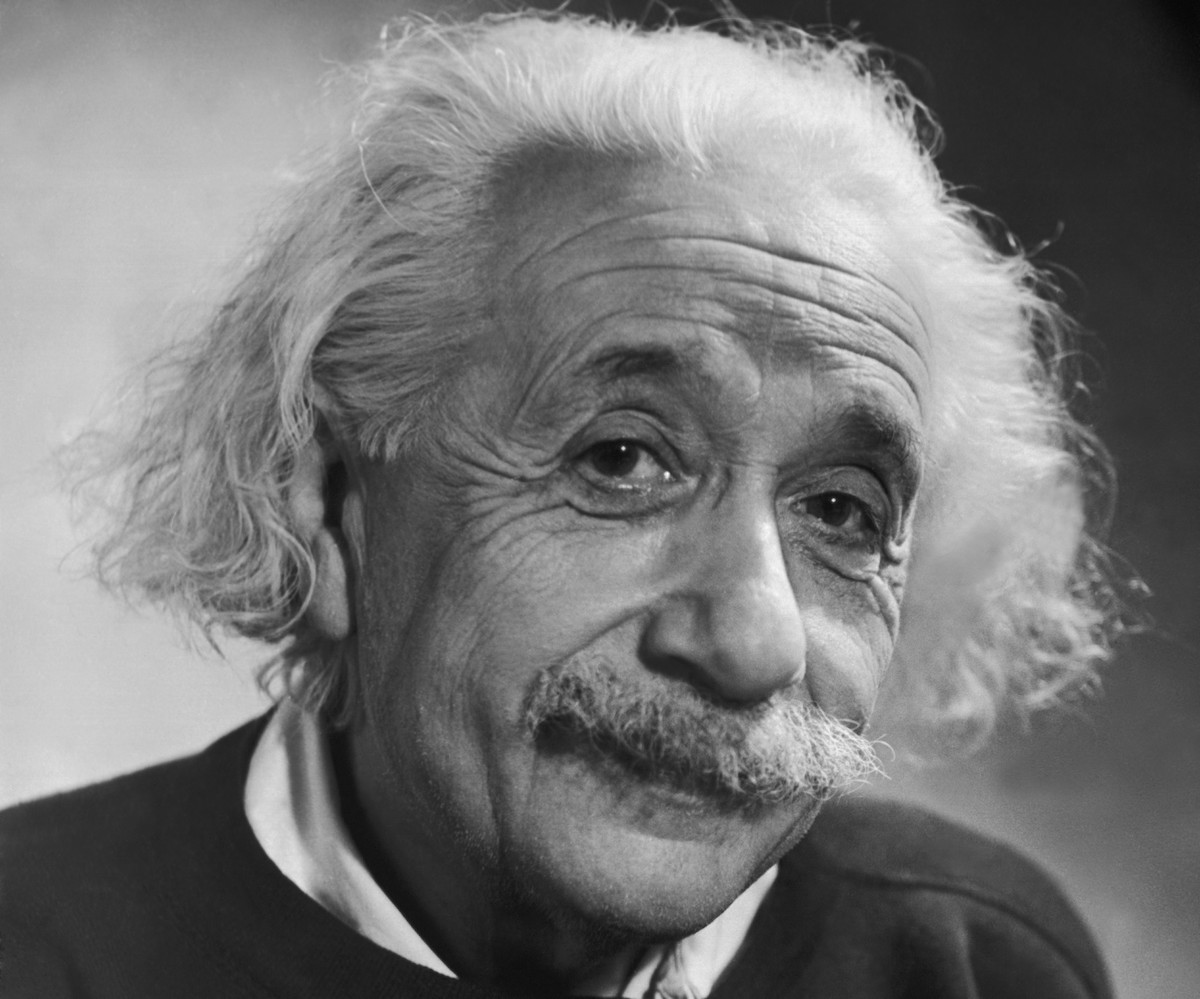
\includegraphics[width=4cm]{images/einstein} \cite{einstein}
\item Beliefs

\begin{itemize}
\item Locality
\item Reality
\end{itemize}
\item QM must be incomplete \cite{EPR}
\item Suggestion: Must be a better `locally real' theory that can describe
nature
\end{itemize}
\end{frame}

\begin{frame}{Asking Nature}

\begin{itemize}
\item John Bell: \\
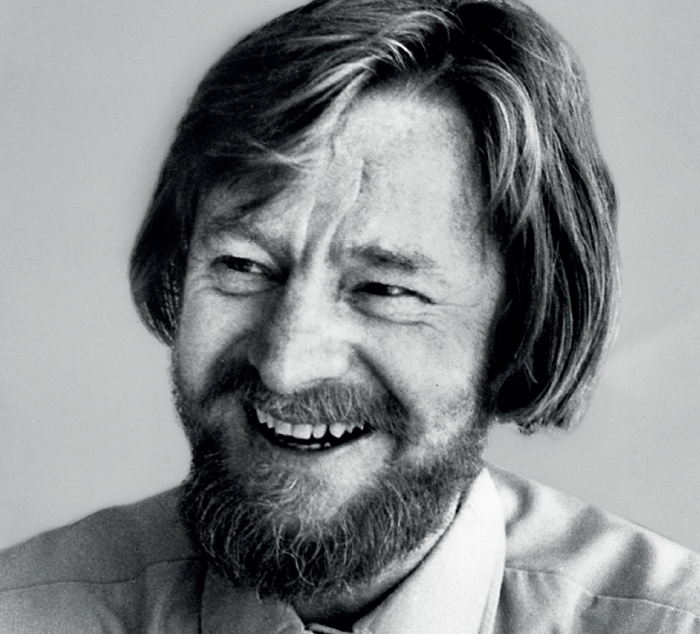
\includegraphics[width=3cm]{images/CCfac8_07_14}\cite{johnBell}
\item Experimental: Can there be a `locally real' theory that conforms with
predictions of QM?\cite{Bell}
\item \emph{NO!}

\begin{itemize}
\item Which assumption is false? - open; progress: Contextuality
\item Can we still do better than QM? - Assume reality but not locality:
DeBroglie Pilot Wave, Bohmian Mechanics
\item Does this mean $\mathbf{q},\mathbf{p}$ don't have `local reality'?
- Reason to believe so
\end{itemize}
\end{itemize}
\end{frame}


\end{section}
\begin{frame}


\Huge{Review/Background}
\end{frame}

\begin{frame}{Bell/CHSH Inequality \cite{CHSH69}}



\begin{itemize}
\item $\left|\left\langle a_{1}(b_{1}+b_{2})+a_{2}(b_{1}-b_{2})\right\rangle \right|\equiv\left|\left\langle \mathcal{B}(a_{i},b_{i})\right\rangle \right|\le2$

\begin{itemize}
\item $\left|a_{i}\right|,\left|b_{i}\right|\le1$
\end{itemize}
\end{itemize}

\pause{}
\begin{itemize}
\item In QM 

\begin{itemize}
\item $\left|\psi\right\rangle \equiv\frac{\left|+-\right\rangle -\left|-+\right\rangle }{\sqrt{2}}$
\end{itemize}

%\pause{}
\begin{itemize}
\item $\hat{z}$, $\hat{x}$, $\hat{z}'=\frac{-\hat{z}-\hat{x}}{\sqrt{2}}$,
$\hat{x}'=\frac{\hat{z}-\hat{x}}{\sqrt{2}}$
\end{itemize}

%\pause{}
\begin{itemize}
\item $\left\langle \mathcal{B}((\hat{x},\hat{z}),(\hat{x}',\hat{z}'))\right\rangle =2\sqrt{2}\nleq2$
\end{itemize}

%\pause{}

\item 
\[
\boxed{\left\langle e^{-i\hat{z}\theta/2}\hat{x}e^{i\hat{z}\theta/2}\otimes e^{-i\hat{z}\phi/2}\hat{x}e^{i\hat{z}\phi/2}\right\rangle =-\cos(\phi-\theta)}
\]

\end{itemize}

%\pause{}


\begin{tabular}{c|c|c|c|c}
\multicolumn{1}{c}{} & \multicolumn{1}{c}{Alice} &  & \multicolumn{1}{c}{Bob} & \tabularnewline
\hline 
Convention & $a_{1}$ & $a_{2}$ & $b_{1}$ & $b_{2}$\tabularnewline
Angle & $\theta{}_{1}=0$ & $\theta{}_{2}=-\pi/2$ & $\phi{}_{1}=3\pi/8$ & $\phi{}_{2}=5\pi/4$\tabularnewline
\end{tabular}

\end{frame}

\begin{frame}{Towards Continuous Variables}

\begin{itemize}
\item Violation

\begin{itemize}
\item Entangled state
\item Measure
\end{itemize}
\item Modular variables
\item Displacement operators
\end{itemize}
\end{frame}

\begin{frame}{Modular Variables}

\begin{itemize}
\item $\hat{p}_{mod}\equiv p_{mod}\left|p\right\rangle \left\langle p\right|$,
$p_{mod}\equiv p\mod(h/L)$
\item $\left|\cos(\hat{p}_{mod}(L/\hbar))\right|\le1$, $\hat{p}_{mod}\leftrightarrow\hat{p}$
\item 
\[
\text{LHS}=\frac{e^{i\hat{p}L/\hbar}+e^{-i\hat{p}L/\hbar}}{2}
\]

\end{itemize}
\end{frame}

\begin{frame}{Displacement Operators}

\begin{itemize}
\item CM: Momentum as a generator of infinitesimal translations
\item $(1-i\hat{p}\frac{\delta L}{\hbar})\left|x\right\rangle =\left|x+\delta L\right\rangle $
\item $(1-i\hat{p}\frac{L}{N\hbar})^{N}\left|x\right\rangle =\left|x+L\right\rangle $
\item $\lim_{N\to\infty}(1-i\hat{p}\frac{L}{N\hbar})^{N}=e^{-i\hat{p}L/\hbar}$
\end{itemize}
\end{frame}

\begin{frame}{Entangled State}
Consider a localized state $\varphi(q) = \braket{q|\varphi}$ symmetric about the position $q=L/2$, where $L\equiv$length scale and $\varphi_n(q)\equiv \varphi(q-nL)$.


\end{frame}


%\end{frame}
\begin{frame}[allowframebreaks]{Bibliography}

\bibliographystyle{plain}
\bibliography{Modular}


\end{frame}
\begin{frame}{Motivation, why bother}

\begin{itemize}
\item Class-room formulation uses spins, an inherently quantum phenomenon 
\end{itemize}

%%\pause{}
\begin{itemize}
\item Extenstion to continuous variables seems simple; position measurement
\end{itemize}

%\pause{}
\begin{itemize}
\item Known: EPR state and displaced parity measurement
\end{itemize}

%\pause{}
\begin{itemize}
\item Issue: Parity is unbounded in phase space
\end{itemize}
\end{frame}

\message{ !name(presBellTestInContVar.tex) !offset(-5) }

\end{document}
